\chapter{Présentation, enjeux et attaques}
\label{chap:constantTimePresentation}


Ce premier chapitre a pour but de présenter les enjeux de la sécurité informatique face aux attaques par canal auxiliaire et d'introduire les attaques temporelles. Nous distinguerons les attaques par canal auxiliaire en deux catégories, montrant ainsi la diversité et les potentiels dangers pour un système sécurisé ignorant de cette menace.



\section{L'exécution du code est observable...}

L'Informatique repose sur deux fondations que l'on tend à distinguer dans l'enseignement : le matériel et le logiciel. Pourtant, si on gardait séparé ces deux domaines, on aurait des tas de piles de métal et de plastiques ou des bibliothèques de livres plein d'idées intéressantes. Au contraire, combiner les les deux parties permet de réaliser des prouesses technologoqies et scientifiques. Ainsi, lorsque l'on conçoit un système sécurisé, il faut prendre en compte ces deux composantes. Or pour implémenter un système sécurisé, il ne faut pas seulement un logiciel sécurisé, il est aussi important que le matériel le soit. Oublier comment fonctionne un support informatique, c'est oublier que programmer se résume à manipuler de l'électricité.\medbreak

Les attaques par canal auxiliaires consistent à exploiter les caractéristiques matériels du support pour gagner en connaissances sur le programme ciblé. Puis exploiter ces connaissances pour acquérir d'avantages d'informations privées : identifiants, clés secrètes, messages personnels. On leurs attribue le terme "canal auxiliaire" car il ne s'agit pas d'essayer de pousser dans ses limites un logiciel ou vérifier que tous les cas particulier sont gérés à travers le canal conçus par le développeur (une interface graphique souvent) mais plutôt de se positionner hors du cadre. Voici quelques travaux présentant une attaque par canal auxiliaire et surtout le canal exploité:
\begin{itemize}
    \item[\cite{DPA_Attack}] Consommation d'énergie 
    \item[\cite{Branch_Attack}] Prédiction de branchement 
    \item[\cite{Thermal_Attack}] Variation de température
    \item[\cite{DRAM_Attack}] Accès à la mémoire DRAM
\end{itemize}\medbreak

Le point commun de ces attaques est la nécéssité d'avoir un point de contact avec la cible. Il faut que l'attaquant puisse récupérer le matériel informatique ou le programme qu'il souhaite attaquer pour ensuite poser des sondes/capteurs enfin d'accumuler de la connaissance et monter son exploitation.\bigbreak


Une autre technique d'attaque consiste à venir introduire une erreur dans le déroulement normal d'un programme. Il s'agit d'une attaque par injection de faute. Originellement \cite{faultOverview} les fautes étaient "naturelles" : un défaut dans le code, un problème avec la transcription vers du code machine, un défaut d'un composant dans le système ou un interférence. Ces interférence sont causées par une irrégularité de l'alimentation électrique, des radiations életromagnétique, une perturbation environnementale \etc\dots
En 2004, \citeauthor{Fault_Attacks} dans leur article \citetitle{Fault_Attacks} \cite{Fault_Attacks} effectuent un tour d'horizon des techniques, montrant l'efficacité de cette méthode sur \indexed{RSA}\footnote{Chiffrement asymétrique par clés secrète du nom de ces auteurs. Standardisé en 1983.}, \indexed{NVM}\footnote{Non Volatile Memory ou mémoire non volatile est un composant informatique qui conservent son contenu en l'absence d'électricité.}, \indexed{DES}\footnote{Algorythme de chiffrement symétrique par bloc. Standardisé en 1977}, \indexed{EEPROM}\footnote{Electrically-Erasable Programmable Read-Only Memory ou mémoire morte effaçable électriquement et programmable.}, \indexed{JVM}\footnote{Machine virtuelle qui exécute des programmes compilés en bytecode Java.}. On y retrouve enfin une liste de contre-mesures et de méthodes de protections contre ces attaques.\medbreak

Ainsi, donner un accès physique à un inconnu est une porte d'entrée pour un attaquant. Pourtant, penser que l'accés physique au support est une condition nécessaire et suffisante pour réaliser une attaque par canal auxiliaire est une erreur.

\section{...à distance}

En effet, il est possible de réaliser des attaques à distance en exploitant d'autres failles de sécurité d'un programme ou d'autres caractéristiques matériels. L'attaque présentée par \citeauthor{LLC_attack} dans \citetitle{LLC_attack} \cite{LLC_attack} repose sur la conception des services clouds où les machines virtuelles accèdent au même matériel. Tandis que la virtualisation crée l'illuson de compartimentation entre les sessions, en réalité, les adresses mémoires pointent vers une ressource physique partagée. Ainsi, l'exploitation du cache du dernier niveau (LLC) permet à un co-hôte de récupérer les clés secrètes d'un autre utilisateur. L'attaquant rempli le cache, puis mesure les temps d'accés vers ces registres. Si des modifications apparaissent dans ces temps, cela signifie que la victime a accédé à ces registres. En répétant cette opération, l'attaquant peut reconstruire les clés secrètes de la victime.\medbreak


D'autres attaques distantes comme celle de \citeauthor{LLC_attack} existent \cite{cryptoeprint:2016/224,Moghimi_2017,vanbulck2018nemesis}, mais on observe rapidement que ces techniques emploient aussi la méthode de chronométrage. En effet, si on cible un algorithme et que l'on mesure son temps d'exécution. Si en fournissant différentes entrées (que l'on considère secrètes) des variations sont observées entre les mesures, alors cela signifie que l'algorithme présente une dépendance à ces entrées. Généralement une sous-fonction de cet algorithme est responsable de ces variations. Cette classe d'attaque est appelée <<\textit{attaque temporelle}>>\footnote{Le terme générique dans la recherche scientifique est <<\textit{time attack}>>. Une traduction plus précise serait <<\textit{attaque par chronométrage}>>. on choisit ici d'utiliser le terme <<\textit{attaque temporelle}>> car il est moins lourd et renvoie directement vers la faille exploitée plutôt que sur la méthode employée.}.\medbreak

Le lien entre temps et exécution de code est connu depuis le début de l'informatique. Le temps est le marqueur de performance, d'efficacité d'un programme. En revanche, l'idée d'exploiter cet indice pour réaliser une attaque est arrivée plus tardivement. \citeauthor{crypto-1996-1469} nous présente le premier, en 1996, comment monter une attaque en utilisant ce canal.\medbreak

Ce lien entre temps et exécution est connu, pourtant la mesure de l'ampleur de la fuite d'information transmise par ce canal n'est pas triviale; ni à son époque, ni à celle-ci.

\begin{listing}[!ht]
    \caption{Exemple de code vulnérable à une attaque temporelle}
    \label{lst:timing_attack_example}
    \begin{minted}[frame=lines,framesep=2mm,baselinestretch=1.2,fontsize=\footnotesize,linenos, gobble=6]{C}
        bool check_pwd(msg, pwd){
        if (msg.length != pwd.length){
            return False
        }
        for(int i = 0; i < msg.length; i++){
            if(msg[i] != pwd[i]){
            return False
            }
        }
        return True
        }
    \end{minted}
\end{listing}
                
Si nous prenons le code présenté par le code \ref{lst:timing_attack_example}, on peut observer que la fonction \texttt{check\_pwd} compare deux chaînes de caractères. Si elles sont de même longueur, elle les compare caractère par caractère. Si elles sont de longueurs différentes, la fonction retourne immédiatement \texttt{False}. Ainsi, si l'on fournit un mot de passe de longueur différente, le temps d'exécution sera constant et court. En revanche, si l'on fournit un mot de passe de même longueur, le temps d'exécution dépendra du nombre de caractères identiques entre les deux chaînes. En effet, la fonction s'arrêtera dès qu'un caractère différent est trouvé. Ainsi, en mesurant le temps d'exécution pour différents mots de passe, un attaquant peut déduire des informations sur le mot de passe correct.\medbreak

On peut synthétiser les éxécutions de la fonction \texttt{check\_pwd} en un graphe comme celui présenté par la figure \ref{fig:timing_attack_example}. Chaque interruption de la fonction peut être observée et mesurée, permettant ainsi de régénérer le mot de passe. Bien sûr la connaissance du protocole cible est requise ou alors il faut réaliser un travail de rétro-ingénierie pour calibrer l'attaque.\medbreak

\begin{figure}[!ht]
    \caption{Suivi du temps d'exécution pour différents mots de passe}
    \label{fig:timing_attack_example}
    \center
    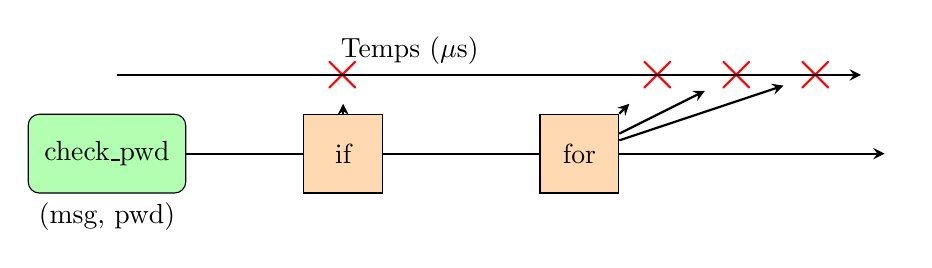
\begin{tikzpicture}[auto]

    % Styles
    \tikzstyle{startstop} = [rectangle, rounded corners, minimum width=2cm, minimum height=1cm, text centered, draw=black, fill=green!30]
    \tikzstyle{process} = [rectangle, minimum width=1cm, minimum height=1cm, text centered, draw=black, fill=orange!30]
    \tikzstyle{arrow} = [thick,->,>=stealth]
    \tikzstyle{arrowred} = [thick,->,>=stealth, draw=red]
    
    % Noeuds
    \node (start) [startstop] {check\_pwd};
    \node (valid) [right of=start, xshift=9cm, green] {\huge{$\checkmark$}};
    \draw [arrow] (start) -- (valid);
    
    \node (inputs) [below of = start, yshift=0.2cm] {(msg, pwd)};
    \node (if) [process] [right of=start, xshift=2cm] {if};
    \node (not) [above of=if, red] {\huge{$\times$}};
    \node (for) [process] [right of=if,, xshift=2cm] {for};
    \node (for1) [above of=for,xshift=1cm, red] {\huge{$\times$}};
    \node (for2) [right of=for1, red] {\huge{$\times$}};
    \node (for3) [right of=for2, red] {\huge{$\times$}};

    \draw [arrow] (if) -- (not);
    \draw [arrow] (for) -- (for1);
    \draw [arrow] (for) -- (for2);
    \draw [arrow] (for) -- (for3);

    \node (t) [above of=start] {};
    \node (a) [above of=valid, xshift=-0.3cm] {};
    \draw [arrow] (t) -- node[above left] {Temps ($\mu$s)} (a.west);
    
    \end{tikzpicture}
\end{figure}

Cette méthode est plus efficace qu'une attaque par force brute. En effet, si l'on suppose que le mot de passe est de 8 caractères de l'alphabet latin. On a alors  256 possibilités par caractère, pour un total de $256^8 = 2^{64}$ possibilités. En revanche, si l'on utilise la méthode de l'attaque temporelle, on peut réduire le nombre de possibilités à $8 + 8 \times 256 = 2056$ possibilités. En effet, on cherche dans un premier temps à identifier la longueur du mot de passe, puis on identifie charactère après charactère pour trouver le bon secret. Avec des temps d'exécution court on est dans les cas de figure d'échec, tandis qu'avec un allongement du temps d'exécution on sait que l'on est sur la bonne piste.\medbreak

Les attaques temporelles présentent la particularité d'être générique. Tandis que les attaques décrites précédemment nécessite des conditions d'accés ou d'initialisation plus importante, cette classse d'attaque présente l'avantage d'être réalisable sur tous les types de systèmes, et notamment les systèmes accessible par internet. La connaissance de cette menace est donc primordiale pour l'implémentation et la mise en service de produit sur internet.\medbreak

Par la suite du document, le terme "fuite" sera utilisé pour désigner un extrait du programme qui peut être exploité pour réaliser une attaque temporelle. Si on reprend le code \ref{lst:timing_attack_example}, les branchement conditionnels ligne [4,6] sont des fuites d'informations. C'est grâce à ces instructions que l'attaque décrite précedemment est réalisable.\medbreak

\textit{Nous allons maintenant nous intéresser aux moyens et méthodes à notre disposition pour se protéger contre les attaques temporelles.}